\section{载流子的散射}
在\xref{sec:载流子的漂移运动}中,我们讨论了载流子的漂移运动以及电导率的问题,但是,这只是讨论了载流子运动的一个方面,具体的说,载流子在外加电场作用下的运动。然而,实际上无论导体或半导体,载流子在电场中的运动远非这样简单,载流子还会发生散射,可以先看看下面的问题。

这是一个很简单的事实:载流子的电场作用下受到电场力,而根据牛顿第二定律,载流子将持续加速,换言之,载流子的漂移速度将持续增大,使电流密度趋于无限大,这显然是荒谬的。

这种矛盾应该如何诠释呢?在一定温度下,晶格上的原子会在格点附近作热振动,晶格中亦有电离了的杂质离子。因此,载流子在半导体中运动时,还会与热振动的晶格原子或是带电的杂质离子发生相互作用,换言之,发生碰撞。碰撞发生后载流子的速度的大小和方向就会发生相应改变,称为\uwave{散射}(Scattering)。因此,我们所谓的“自由”载流子,其“自由”实际上仅存在于两次散射之间,换言之,每次碰撞都将清除载流子原有的速度状态,这也就是为何电场对载流子的作用无法无限积累的原因,\empx{载流子的漂移速度,仅是两次碰撞间电场的作用结果}
\begin{itemize}
    \item 将两次散射间自由运动的平均路程,定义为\uwave{平均自由程}(Mean Free Path)。
    \item 将两次散射间自由运动的平均时间,定义为\uwave{平均自由时间}(Mean Free Time)。
\end{itemize}
现在已经弄清什么是散射了,那么,什么会导致散射?我们散射的发生机理称为\uwave{散射机构}。

\subsection{电离杂质的散射}
施主杂质电离后是一个带正电的离子,受主杂质电离后是一个带负电的离子,在电离施主或受主周围将形成一个库伦势场,这一库伦场局部破坏了杂质附近的周期性势场。当载流子运行到杂质离子附近时,受到库伦场的作用,运动方向将会发生改变,以$\vb*{v}$接近,以$\vb*{v'}$远离。
\begin{Figure}[电离杂质散射]
    \begin{FigureSub}[电离施主散射]
        \includegraphics[scale=1]{build/Chapter04B_01.fig.pdf}
    \end{FigureSub}
    \hspace{3cm}
    \begin{FigureSub}[电离受主散射]
        \includegraphics[scale=1]{build/Chapter04B_02.fig.pdf}
    \end{FigureSub}
\end{Figure}

如\xref{fig:电离杂质散射}所示,注意到,电离杂质散射时载流子的散射轨迹是一个双曲线,杂质离子位于双曲线的某一个焦点,异号载流子沿靠近焦点的轨迹散射,同号载流子沿远离焦点的轨迹散射。

我们常用\uwave{散射概率}(Scatter Probability)描述散射的强弱,记作$P$,代表单位时间内一个载流子散射的次数。分析表明,浓度为$N_i$的电离杂质对散射概率$P_\text{i}$与温度的关系满足下式。
\begin{BoxFormula}[电离杂质的散射概率]
    电离杂质的散射概率满足
    \begin{Equation}
        P_\text{i}\propto N_\text{i}T^{-3/2}
    \end{Equation}
\end{BoxFormula}

根据\fancyref{fml:电离杂质的散射概率}
\begin{itemize}
    \item 电离杂质的浓度越高,载流子遭受散射的机会就多,故$P_\text{i}$越大。
    \item 温度越高,载流子热运动的平均速度就越大,可以较快掠过杂质离子,故$P_\text{i}$越小。
\end{itemize}

\subsection{晶格振动的散射}
晶格原子的振动产生的波称为\uwave{格波}(Lattice Wave)。在固体物理中我们已经非常深刻的学习过晶格振动和格波理论,因此,在半导体物理中,我们只是简要的回顾一下相关结论,以便讨论它们对载流子的散射作用。我们知道,电子波波矢以$\vb*{k}$表示,格波波矢则以$\vb*{q}$表示,以示区分。根据固体物理的知识,若每个原胞有$r$个原子,则格波的色散关系$\omega_\text{a}(\vb*{q})$有$3r$组,即有$3r$支格波,并且,其中$3$支为声频支,剩余$3r-3$支为光频支。而对于硅、锗、\Romnum{3}--\Romnum{5}族化合物半导体,原胞中大多只有$2$个原子,因此,半导体有$6$支格波,声频和光频各$3$支。

\begin{Figure}[金刚石的格波色散关系]
    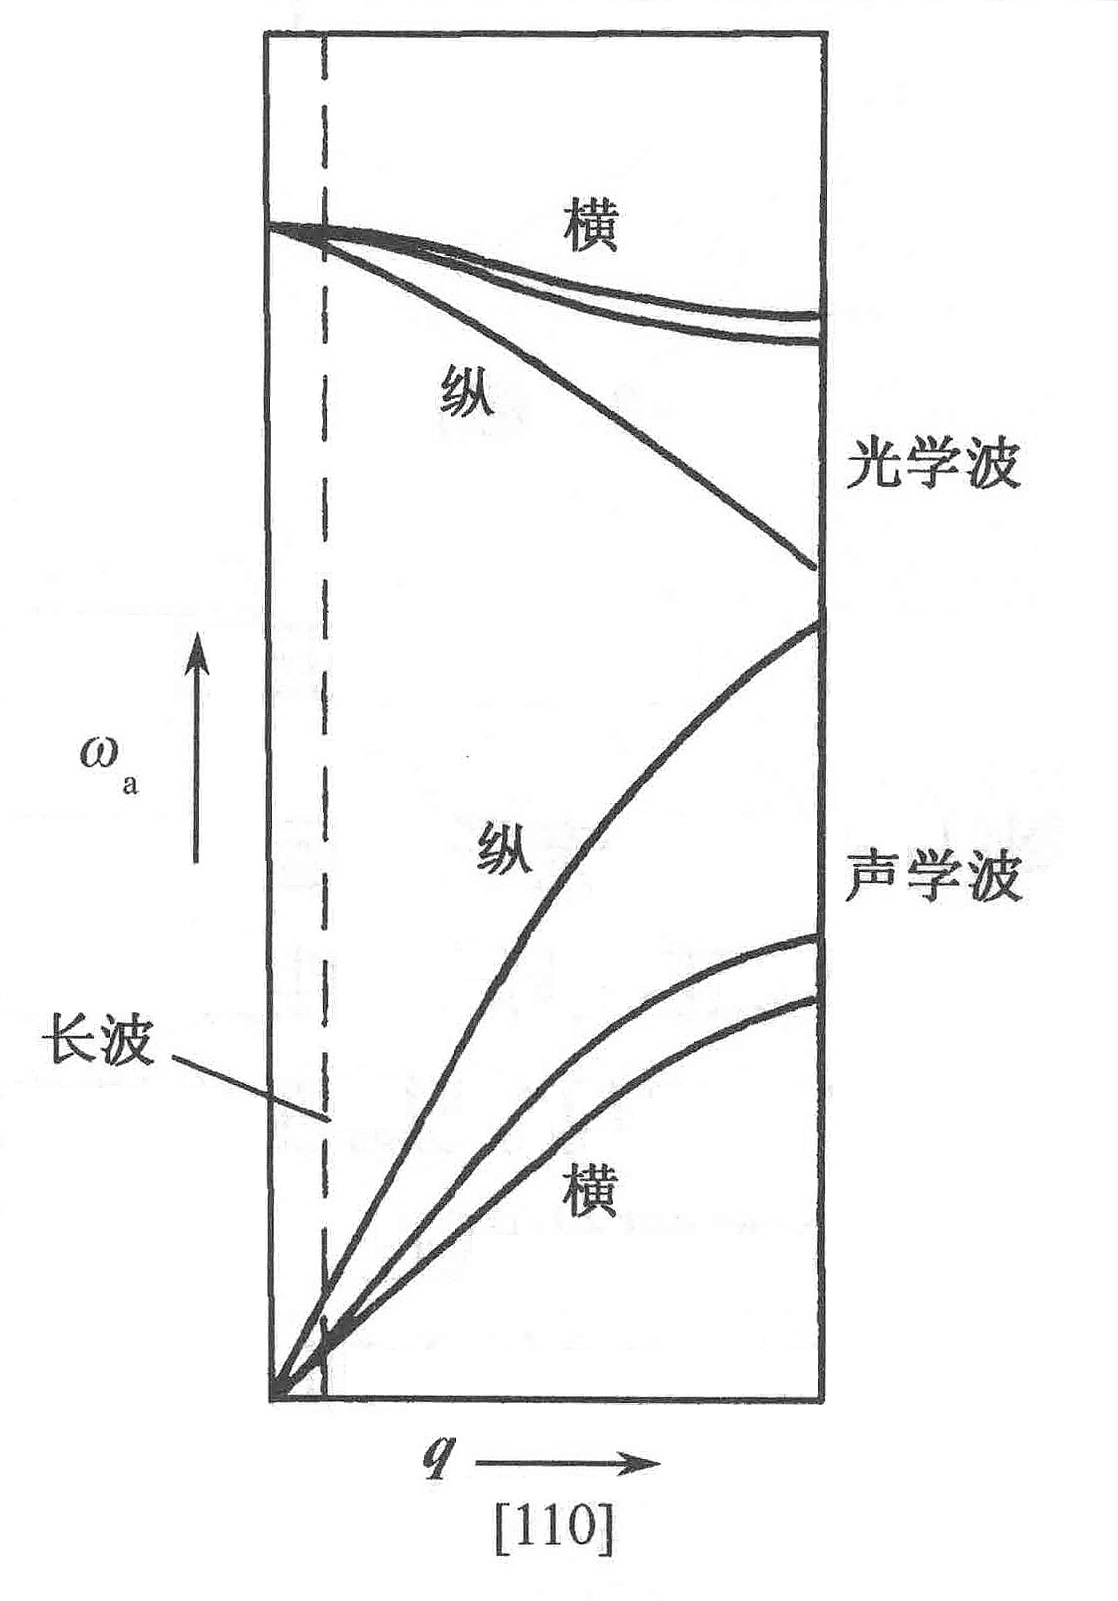
\includegraphics[width=4.5cm]{image/Lattice_Omega_Q.jpg}
\end{Figure}

如\xref{fig:金刚石的格波色散关系}所示,对于金刚石结构的半导体
\begin{itemize}
    \item 频率较低的三支是声频波,其中,较低的两支是横波,较高的一支是纵波。
    \item 频率较高的三支是光频波,其中,较高的两支是横波,较低的一支是纵波。
\end{itemize}
声频支格波和光频支格波在振动方式上也存在显著差异,如\xref{fig:声频支和光频支的长波特性}所示,在长波范围内,声学波的频率与波矢成正比,因此,声学波的行为近似于连续介质中的弹性波。光学波的频率则近似为一个常数,并且,光学波的相邻两个原子总是以相反的方向运动,与弹性波非常不同。

\begin{Figure}[声频支和光频支的长波特性]
    \begin{FigureSub}[声频支的长波特性]
        \includegraphics[scale=0.76]{build/Chapter04B_03.fig.pdf}
    \end{FigureSub}\vspace{0.75cm}
    \begin{FigureSub}[光频支的长波特性]
        \includegraphics[scale=0.76]{build/Chapter04B_04.fig.pdf}
    \end{FigureSub}
\end{Figure}

实际上,角频率为$\omega_\text{a}$的一个格波,其能量也是量子化的,只能取
\begin{Equation}
    \frac{1}{2}\hbar\omega_\text{a},~~
    \frac{3}{2}\hbar\omega_\text{a},~~
    \frac{5}{2}\hbar\omega_\text{a},~~ 
    \cdots,~~ 
    \qty(n+\frac{1}{2})\hbar\omega_\text{a}
\end{Equation}
因此,格波的能量是以$\hbar\omega_\text{a}$为单元的。晶格与电子交换能量时,晶格原子的振动状态就要发生改变,换言之,格波能量就要发生变化,但由于格波能量变化只能是$\hbar\omega_\text{a}$的整数倍,因此我们就将格波的能量子$\hbar\omega_\text{a}$称为\uwave{声子}(Phonon),并且,我们将能量为$(n+1/2)\hbar\omega_\text{a}$的格波解释为$n$个属于这一格波的声子(频率$\omega_\text{a}$不同的格波的声子是不同的),同时
\begin{itemize}
    \item 当格波能量减少$\hbar\omega$时,就称格波放出一个声子。
    \item 当格波能量增加$\hbar\omega$时,就称格波吸收一个声子。
\end{itemize}
声子的说法不仅生动的表现出格波能量的量子化,而且在分析晶格与物质间的相互作用时很方便。例如,我们或许会很难想象电子与一大堆来回振动的晶格原子发生相互作用,但电子和某种称为声子的准粒子碰撞则是容易理解的,即,\empx{晶格振动的散射,即电子与声子的碰撞}。

根据玻尔兹曼统计理论,在温度$T$时频率为$\omega_\text{a}$的格波的平均能量为
\begin{Equation}
    \bar{E}=\frac{1}{2}\hbar\omega_\text{a}+\qty(\frac{1}{\exp(\hbar\omega_\text{a}/\kB T)-1})\hbar\omega_\text{a}
\end{Equation}
亦可以记为
\begin{Equation}
    \bar{E}=\frac{1}{2}\hbar\omega_\text{a}+\bar{n_\text{q}}\hbar\omega_\text{a}
\end{Equation}
其中$n_\text{q}$按照上述论述,可以解释为平均声子数
\begin{BoxFormula}[平均声子数]
    在温度$T$下,平均声子数满足
    \begin{Equation}
        \bar{n_\text{q}}=\frac{1}{\exp(\hbar\omega_\text{a}/\kB T)-1}
    \end{Equation}
\end{BoxFormula}

电子和声子的碰撞也遵循动量守恒和能量守恒,基于此,我们来讨论电子的晶格振动散射。

设散射前后,电子的波矢和能量分别为$\vb*{k},\vb*{k}'$和$E,E'$,依据动量守恒和能量守恒\setpeq{电子的晶格振动散射}
\begin{Gather}
    \hbar\vb*{k}'-\hbar\vb*{k}=\pm\hbar\vb*{q}\xlabelpeq{1}\\
    E'-E=\pm\hbar\omega_\text{a}\xlabelpeq{2}
\end{Gather}
这里两式只能取$\pm\hbar\vb*{q}$和$\pm\hbar\omega_\text{a}$的原因是,在电子和晶格相互作用时,通常发生的都是单声子过程,换言之,总是只有一个声子被吸收或发射。以上,以正号表示吸收,以负号表示发射。

若散射角,即$\vb*{k},\vb*{k}'$的夹角为$\theta$,则依照余弦定理
\begin{Equation}&[3]
    q^2=k^2+k'^2-2kk'\cos\theta
\end{Equation}
稍作整理
\begin{Equation}&[4]
    q^2=(k-k')^2-2kk'(1-\cos\theta)
\end{Equation}
散射前后电子波矢的大小通常可以近似相等,即$k=k'$,故
\begin{Equation}&[5]
    q^2=2k^2(1-\cos\theta)=4k^2\sin^2\frac{\theta}{2}
\end{Equation}
即
\begin{Equation}&[6]
    q=2k\sin\frac{\theta}{2}
\end{Equation}
设电子速度的大小在散射前后均为$v$,将电子动量以经典形式表示
\begin{Equation}&[7]
    \hbar k=\mne v
\end{Equation}
设声子速度的大小为$u$,由于长声学波类似弹性波,故$\omega_\text{a}=qu$,因而
\begin{Equation}&[8]
    \hbar\omega_\text{a}=\hbar qu
\end{Equation}
这样,将\xrefpeq{8},\xrefpeq{6},\xrefpeq{7}连续代入\xrefpeq{2}
\begin{Equation}
    \delt{E}=E'-E=\hbar\omega_\text{a}=\hbar qu=2\hbar k u\sin\frac{\theta}{2}=2\mne uv\sin\frac{\theta}{2}
\end{Equation}
或者
\begin{Equation}
    \delt{E}=2\mne v^2\qty(\frac{u}{v})\sin\frac{\theta}{2}
\end{Equation}
由此可见,由于声子的速度$u$很小,因此,对于长声学波而言$\delt{E}\approx 0$,即散射前后电子能量基本不变,称为弹性散射,对于长光学波而言,以上讨论并不适用,但明显的是,由于光学波的声子能量$\hbar\omega_\text{a}$较大(由于$\omega_\text{a}$较大),故散射前后电子能量有较大改变,称为\uwave{非弹性散射}。

\subsubsection{声学波散射}
声学波中,纵声学波产生体变,横声学波产生切变,两者都可以一定程度的影响能带极值的变化,使能带结构出现波形起伏。这是为什么呢?以纵声学波为例,其传播将使得原子分布出现疏密变化,疏处体积膨胀,密处体积压缩,这将使得依赖原子间距的的禁带宽度随疏密变化发生起伏,进而使得能带结构出现起伏。通常来说,纵声学波在散射中占据主导地位,横声学波的切变仅对能带具有多极值(具有椭球等能面)的硅和锗中的载流子,才有一定散射作用。

声学波的散射概率适用下式。
\begin{BoxFormula}[声学波的散射概率]
    声学波的散射概率满足
    \begin{Equation}&[A]
        P_\text{s}\propto T^{3/2}
    \end{Equation}
    更具体的表达是(以对导带电子的散射为例)\footnote[2]{这里电子热运动的速度$v\propto T^{1/2}$,因此有上式。}
    \begin{Equation}&[B]
        P_\text{s}=\frac{\varepsilon_\text{c}^2\kB T(\mne)^2}{\pi\rho\hbar^4u^2}v
    \end{Equation}
    其中,$\rho$为晶格密度,$u$为波速,$\varepsilon_\text{c}$为形变势常数。\footnote[3]{参见\xref{subsec:线缺陷}中的\xrefpeq[线缺陷]{1}。}
\end{BoxFormula}


\subsubsection{光学波散射}
光学波与离子晶体密切相关,因为正负离子在振动时的位移方向相反,这恰于\xref{fig:光频支的长波特性}中描绘的光学波的特性相符。光学波在传播时,以纵光学波为例,如果我们只看其中一种离子,那它和纵声学波一样也是形成疏密相间的区域,而由于正负离子的位移方向相反
\begin{itemize}
    \item 正离子的密区与负离子的疏区相重合,在该半波长区带正电。
    \item 负离子的密区与正离子的疏区相重合,在该半波长区带负电。
\end{itemize}
这就会产生一个附加的电场,从而对载流子实现散射。光学波的散射概率适用下式。
\begin{BoxFormula}[光学波的散射概率]*
    光学波的散射概率满足
    \begin{Equation}&[A]
        P_\text{o}\propto\qty[\exp(\hbar\omega_\text{l}/\kB T)-1]^{-1}
    \end{Equation}
    更准确的描述是
    \begin{Equation}&[B]
        P_\text{o}\propto\frac{(\hbar\omega_\text{l})^{3/2}}{(\kB T)^{1/2}f(\hbar\omega_\text{l}/\kB T)}\frac{1}{\exp(\hbar\omega_\text{l}/\kB T)-1}
    \end{Equation}
    其中,$\omega_\text{l}$为纵声学波的频率,$f$是一个值在$0.6\sim 1.0$内的函数。
\end{BoxFormula}
光学波的散射概率,主要取决于\xrefpeq{A}中的指数因子$\qty[\exp(\hbar\omega_\text{l}/\kB T)-1]^{-1}$,不难注意到,这里的指数因子,其实就是\xref{fml:平均声子数}中定义的平均声子数$\bar{n_\text{q}}$,我们看到,随着温度$T$的降低平均声子数$\bar{n_\text{q}}$迅速减小,使得光学波的散射概率$P_\text{o}$也迅速减小,这说明了两点,第一是至少得有声子才能发生吸收声子的散射,第二是光学波的散射在低温时不起什么作用,可以忽略。

光学波在\Romnum{4}--\Romnum{6}族的离子化合物(例如硫化铅)和部分\Romnum{3}--\Romnum{5}族带有离子键成分的共价化合物(例如砷化镓)中有重要的散射作用。温度较高时,光学波在硅锗中也有一定的散射作用。

这里我们总结一下
\begin{itemize}
    \item 硅和锗等原子半导体中,以电离杂质散射和声学波散射为主。
    \item 化合物半导体中,同时存在电离杂质散射、声学波散射、光学波散射。
\end{itemize}